%\iffalse
\let\negmedspace\undefined
\let\negthickspace\undefined
\documentclass[journal,12pt,twocolumn]{IEEEtran}
\usepackage{cite}
\usepackage{amsmath,amssymb,amsfonts,amsthm}
\usepackage{algorithmic}
\usepackage{graphicx}
\usepackage{textcomp}
\usepackage{xcolor}
\usepackage{txfonts}
\usepackage{listings}
\usepackage{enumitem}
\usepackage{mathtools}
\usepackage{gensymb}
\usepackage{comment}
\usepackage[breaklinks=true]{hyperref}
\usepackage{tkz-euclide} 
\usepackage{listings}
\usepackage{gvv}                                        
\def\inputGnumericTable{}                                 
\usepackage[latin1]{inputenc}                                
\usepackage{color}                                            
\usepackage{array}                                            
\usepackage{longtable}                                       
\usepackage{calc}                                             
\usepackage{multirow}                                         
\usepackage{hhline}                                           
\usepackage{ifthen}                                           
\usepackage{lscape}

\newtheorem{theorem}{Theorem}[section]
\newtheorem{problem}{Problem}
\newtheorem{proposition}{Proposition}[section]
\newtheorem{lemma}{Lemma}[section]
\newtheorem{corollary}[theorem]{Corollary}
\newtheorem{example}{Example}[section]
\newtheorem{definition}[problem]{Definition}
\newcommand{\BEQA}{\begin{eqnarray}}
\newcommand{\EEQA}{\end{eqnarray}}
\newcommand{\define}{\stackrel{\triangle}{=}}
\theoremstyle{remark}
\newtheorem{rem}{Remark}

\begin{document}

\bibliographystyle{IEEEtran}
\vspace{3cm}
\title{\textbf{10.05.2}}
\author{EE23BTECH11053-R.Rahul$^{*}$% <-this % stops a space
}

\maketitle

\textbf{QUESTION:}\\
1. In the following APs, find the missing terms in the boxes:\\
(i) $ 2,\boxed{}, 26 $\\
(ii)$\boxed{} , 13,\boxed{} , 3$\\
(iii)$ 5,\boxed{} ,\boxed{} ,$9\(\frac{1}{2}\)$\\$
(iv)$'- 4',\boxed{} ,\boxed{} ,\boxed{} ,\boxed{} , 6$\\
(v) $\boxed{}, 38,\boxed{} , \boxed{}, \boxed{}, '- 22'$\\

\textbf{Solution:}\\


\begin{table}[h]
  \centering
  \begin{tabular}{|c|c|c|c|c|c| }
    \hline
    \(n\) & \(x_1(n)\)& \(x_2(n)\) & \(x_3(n)\) & \(x_4(n)\) & \(x_5(n)\) \\
    \hline
    0 & 2  & 18 &  5  &  -4  &  53  \\
    1 & 14 & 13 & $6\frac{1}{2}$ & -2 & 38 \\
    2 & 26 & 8 & 8 & 0 & 23 \\
    3 & 38 & 3 & $9\frac{1}{2}$ & 2 & 8 \\
    4 & 50 & -2 & 11 & 4 & -7 \\
    5 & 62 & -7 & $12\frac{1}{2}$ & 6 & -22 \\
    \hline
  \end{tabular}
  \caption{first three terms of AP series}
  \label{tab:xn}
\end{table}





     (i) $a_1$=2 ,$a_3$=26, $a_3$=$a+2d$\\
     \begin{align}
          26&=2+2d\\
        24&=2d \\
        \therefore d&=12\\
        a_2&=14
     \end{align}
       
         \vspace{0.25cm}
         
     (ii) $a_2=13, a_4=3 , a_2=a+d, a_4=a+3d$\\ 
     \begin{align}
         3-13&=2d\\
           -10&=2d\\
           \therefore d&=-5\\
            a_1&=18\\
            a_3&=8
     \end{align}
            \vspace{0.25cm} 
          
     (iii)$a_1$=5, $a_4$=9\(\frac{1}{2}\) , $a_4=a+3d$\\
     \begin{align}
           9\ \frac{1}{2}\ &=5+3d \\
           3d&=4\frac{1}{2}\\
           \therefore d&=1\ \frac{1}{2}\ \\ 
          a_2&=6\ \frac{1}{2}\\
          a_3&=8
     \end{align}
          \vspace{0.25cm} 
          
     (iv) $a_1$=-4 , $a_6$=6, $a_6$=a+5d\\
\begin{align}
     6&=-4+5d\\
     10&=5d\\
     \therefore d&=2\\
          a_2&=-2\\
          a_3&=0\\
          a_4&=2\\
          a_5&=4
\end{align}
          \\ \vspace{0.25cm} 
          
     (v)  $a_2$=38 $a_6$=-22 \\
     \begin{align}
         -22-38&=4d\\
          -60&=4d\\
           \therefore d&=-15\\
            a_1&=53\\
            a_3&=23\\
            a_4&=8\\
            a_5&=-7\\
     \end{align}
             
          


\begin{enumerate}
 \item 
The $Z$-transform of $x(n) = 2 + 12n$ is given by:
\begin{align}
    &X(z)= \sum_{n=-\infty}^{\infty} x(n) u(n)z^{-n}\\
    &X(z) = \sum_{n=-\infty}^{\infty} (2+12n) u(n)z^{-n}\\
    &X(z)=2 \frac{1}{1-{z^{-1}}}+ 12\frac{z^{-1}}{(1-{z^{-1}})^2}\\
    &X(z)=\frac{2+{10z^{-1}}}{(1-{z^{-1}})^2}  \qquad|z|>1 \\
\end{align}
\item
The $Z$-transform of $x(n) = 18 - 5n$ is given by:

\begin{align}
    &X(z) = \sum_{n=-\infty}^{\infty} x(n) u(n)z^{-n}\\
    &X(z) = \sum_{n=-\infty}^{\infty} (18-5n) u(n)z^{-n}\\
    &X(z)=18 \times \frac{1}{1-{z^-1}} - 5\frac{z^{-1}}{(1-{z^-1})^2}\\
    &X(z)=\frac{18-{23z^{-1}}}{(1-{z^{-1}})^2} \qquad  |z|>1 \\
\end{align}
\item 
$Z$-transform of $x(n) = 5 + \frac{3}{2}n$ is given by:

\begin{align}
    &X(z) = \sum_{n=-\infty}^{\infty} x(n) u(n)z^{-n} \\
    &X(z) = \sum_{n=-\infty}^{\infty} (5+\frac{3}{2}n) u(n)z^{-n} \\
    &X(z)=5 \times \frac{1}{1-{z^{-1}}}+ \frac{3}{2}\frac{z^{-1}}{(1-{z^{-1}})^2}\\
    &X(z)=\frac{5-\frac{7}{2}{z^{-1}}}{(1-{z^{-1}})^2} \qquad |z|>1\\
\end{align}
\item 

\vspace{2cm}
$Z$-transform of $x(n) = -4 + 2n$ is given by:

\begin{align}
       &X(z) = \sum_{n=-\infty}^{\infty} x(n) u(n)z^{-n} \\
       &X(z) = \sum_{n=-\infty}^{\infty} (-4 + 2n) u(n)z^{-n} \\
       &X(z)=-4 \times \frac{1}{1-{z^{-1}}}+ 2 \frac{z^{-1}}{(1-{z^{-1}})^2}\\
       &X(z)=\frac{-4+6{z^{-1}}}{(1-{z^{-1}})^2} \qquad  |z|>1\\
\end{align}
\item 
$Z$-transform of $x(n) = 53 - 15n$ is given by:

\begin{align}
       &X(z) = \sum_{n=-\infty}^{\infty} x(n) u(n)z^{-n} \\
       &X(z) = \sum_{n=-\infty}^{\infty} (53 - 15n) u(n)z^{-n} \\
       &X(z)=53 \times \frac{1}{1-{z^{-1}}}- 15\frac{z^{-1}}{(1-{z^{-1}})^2}\\
       &X(z)=\frac{53-68{z^{-1}}}{(1-{z^{-1}})^2}\qquad|z|>1\\
\end{align}
\end{enumerate}

\begin{figure}[h]
       \vspace*{-1cm}
       \centering
        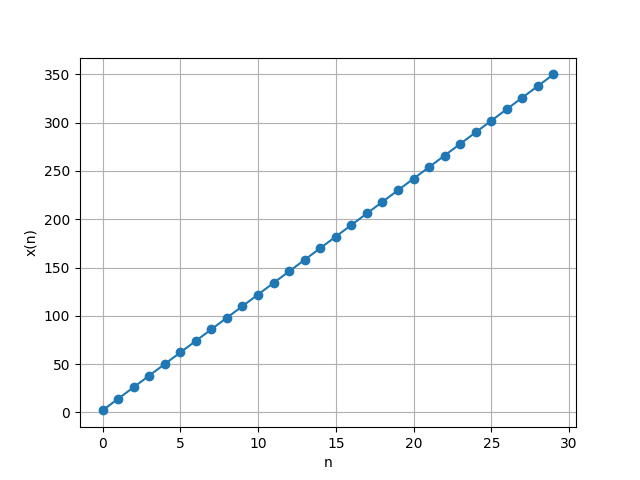
\includegraphics[width=0.8\linewidth]{figs/download.png} % Adjust the width as needed
        \caption{}
\end{figure}

\begin{figure}[h]
      \vspace*{-1cm}
      \centering
       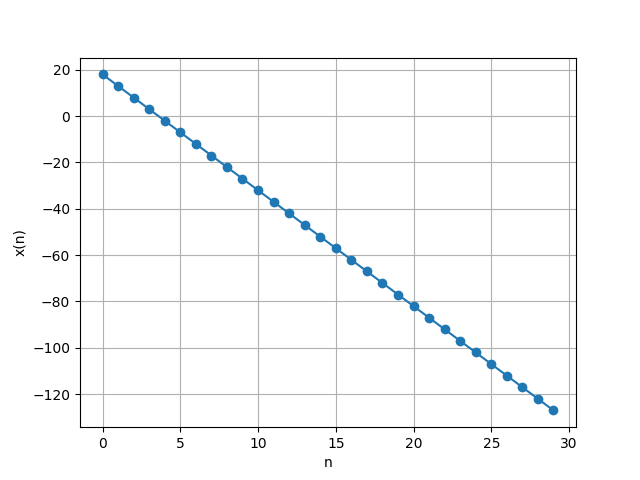
\includegraphics[width=0.8\linewidth]{figs/download (1).png} % Adjust the width as needed
        \caption{}
    \end{figure}
    
\begin{figure}[h]
      \vspace*{-2cm}
      \centering
       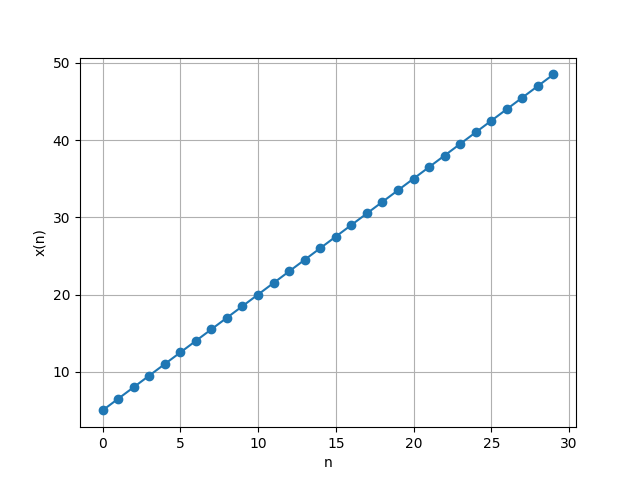
\includegraphics[width=0.8\linewidth]{figs/download (2).png} % Adjust the width as needed
        \caption{}
    \end{figure}
    
\begin{figure}[h]
      \vspace*{-2cm} 
      \centering
       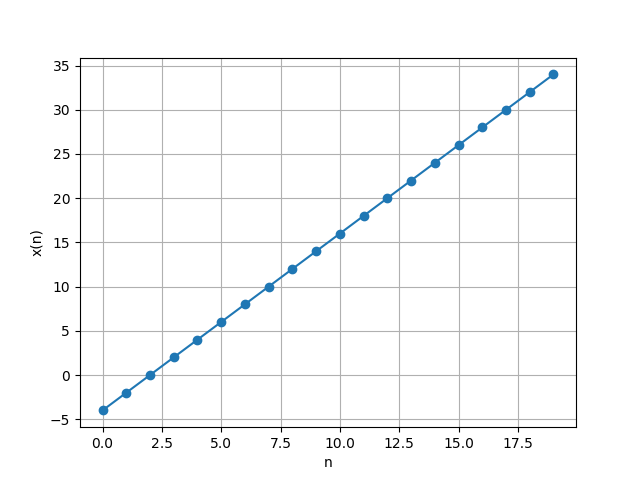
\includegraphics[width=0.8\linewidth]{figs/download (3).png} % Adjust the width as needed
        \caption{}
    \end{figure}
    
\begin{figure}[h]
      \vspace{-2cm}
      \centering
       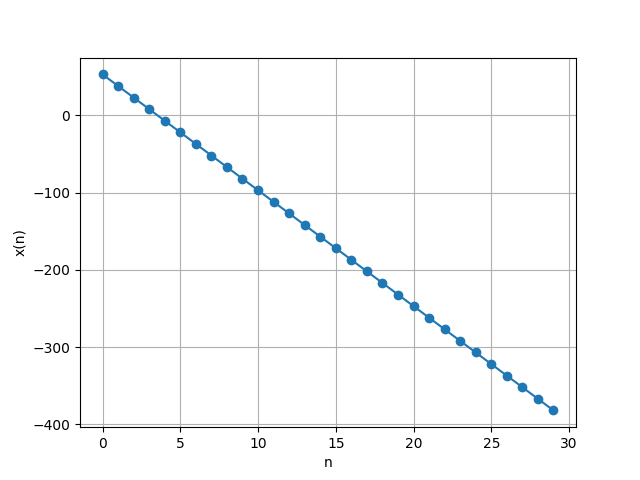
\includegraphics[width=0.8\linewidth]{figs/download (4).png} % Adjust the width as needed
        \caption{}
\end{figure}


\end{document}
